%!TEX program = xelatex
%!TEX root = ./thesis.tex
\chapter{Experiments}
%!TEX program = xelatex
%!TEX root = ./thesis.tex

\section{Experiments on the Basic Task \textit{move0}}\label{sec_exp_move0}

The methods for solving the basic task move0 are discussed in this section.

First, we would like to verify the ability to reproducing consistent learning performance discussed in~\cite{henderson2017matters}. We choose the ACKTR~\cite{wu2017scalable} method and test it on the move0 task. As is discussed previously, the move0 task is actually a single-modal environment since the image observation is redundant. Separate neural network parameters are used for the actor network and critic network. The neural networks have the same architecture that consists of two fully connected layers with 64 hidden units after the motion sensor input. The neural network outputs the mean parameter of the policy distribution. The standard deviation of the policy distribution is parameterized by an independent parameter vector. The batch-size is set to 8000, the KL-divergence set to 0.0001 and 20 parallel agents are used to generate experience. The resulting learning performance is shown in Figure~\ref{fig_acktr_reprod}. It appears that the performance of one experiment gets stuck at a score below 3000 while another continues to improve after reaching the score of 4000. 
\begin{figure}[!htbp]
	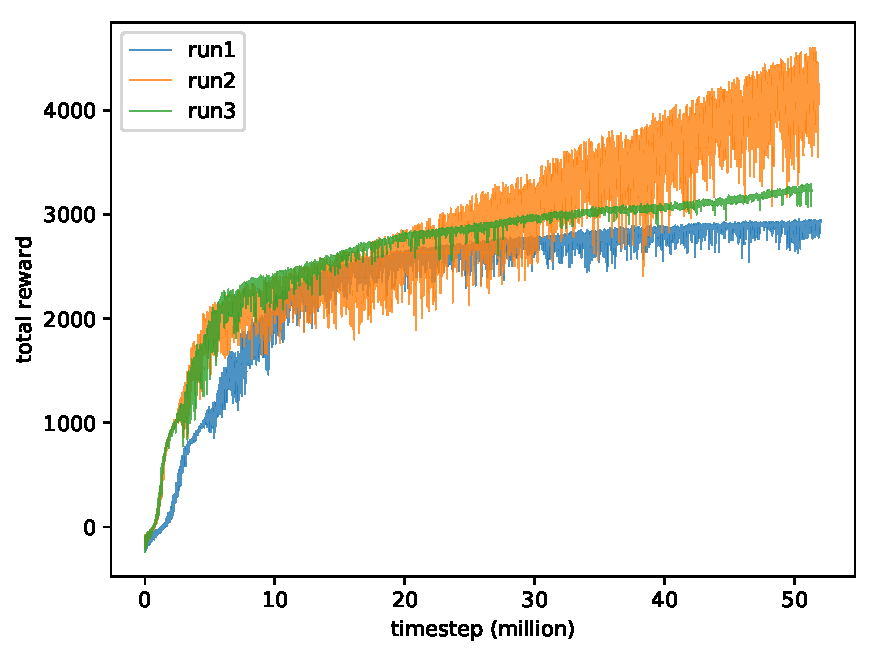
\includegraphics[width=0.7\textwidth]{images/rec_0403_reprod}
	\centering
	\caption{Inconsistent performance produced by ACKTR agents with the same  parameters but different runs. The vertical axis is the total return averaged over the recent 20 episodes and the horizontal axis is the number of million time-steps}\label{fig_acktr_reprod}
\end{figure}

We'd also like to compare the learning performance of the ACKTR method across different learning rates. The experiment result showing the performance of the original ACKTR algorithm with different learning rates is shown in Figure~\ref{fig_acktr_mom_tune}. The result shows that the agents are likely to get stuck at the score of around 3000. 
%The reason might be that while the KL-divergence based trust-region method provides a theoretical guarantee on the monotonic improvement of performance, the agent might converge too early at local minimums and fails to make efficient exploration.
\begin{figure}[!htbp]
	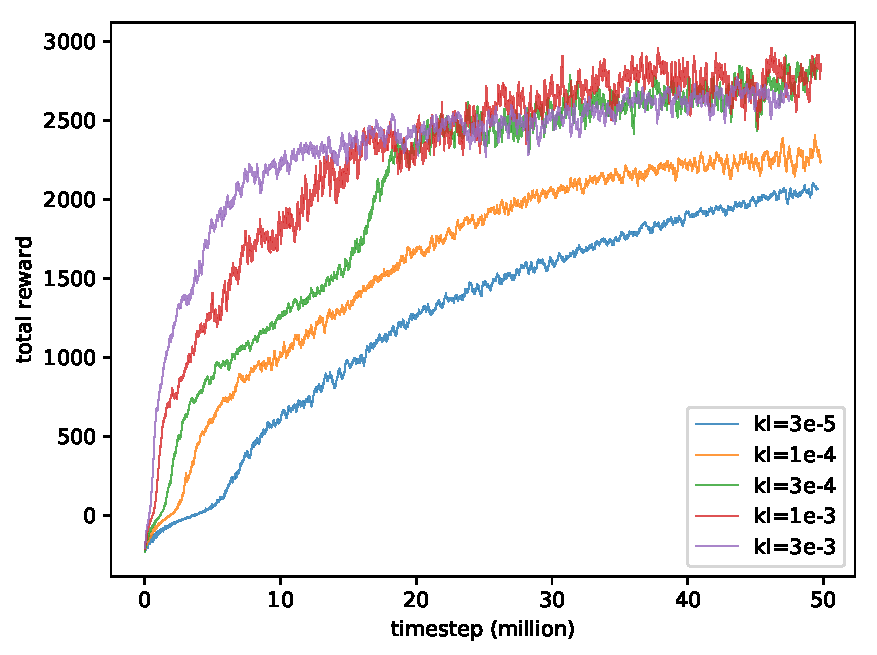
\includegraphics[width=0.7\textwidth]{rec_180521_acktr_mom}
	\centering
	\caption{Performance of ACKTR agents with different KL-divergence constraints. All the agents are trained with batch-size 4000 and 20 parallel agents. The vertical axis is the total return averaged over the recent 200 episodes and the horizontal axis is the number of million time-steps}\label{fig_acktr_mom_tune}
\end{figure}

We'd also like to verify if the proposed W-KTR method is less prone to local minimums on the task move0. The experiment results comparing the performance of W-KTR agents with different learning rates is shown in Figure~\ref{fig_wass_const_tune}. The result shows that none of the W-KTR agents gets stuck at the local minimum around 3000, and their final performance can reach a total return of around 6000. However, the W-KTR agent appears to have a much slower rate of improvement on the performance before 50 million time-steps.
\begin{figure}[!htbp]
	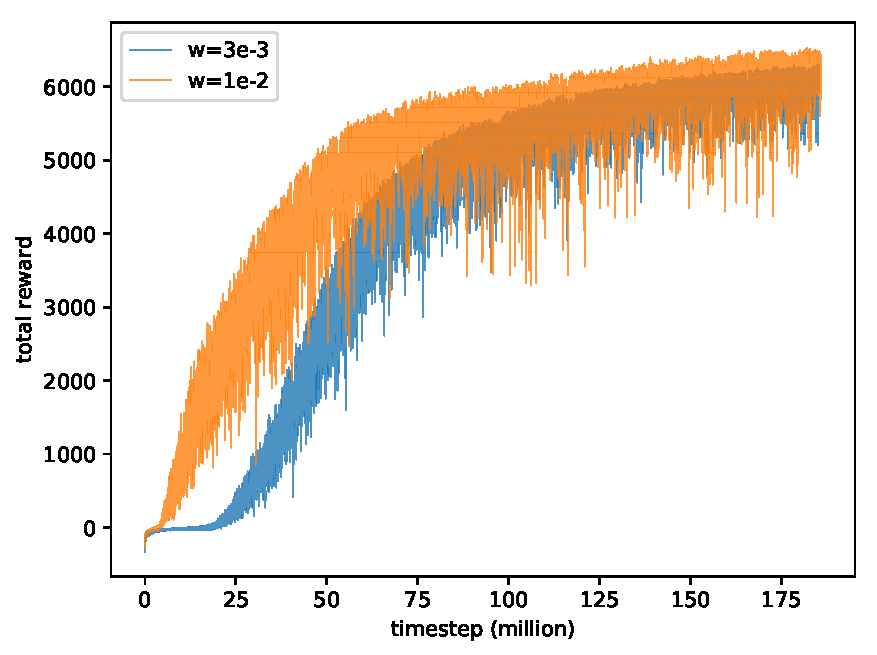
\includegraphics[width=0.7\textwidth]{rec_180608_wass_const}
	\centering
	\caption{Performance of W-KTR agents with different W2-metric constraints. All the agents are trained with batch-size 4000 and 20 parallel agents. The vertical axis is the total return averaged over the recent 20 episodes and the horizontal axis is the number of million time-steps}\label{fig_wass_const_tune}
\end{figure}

We also test if applying a decaying Wasserstein constraint at the early phase of training will improve the learning performance. The experiment of a W-KTR agent with a decaying W-2 constraint from 0.02 to 0.00003 in the first 15 million time-steps is shown in Figure~\ref{fig_wass_decay}. The agent can achieve a more efficient learning performance in the first 50 million time-steps. However, the drawback of this method is that more hyper-parameters need to be tuned.
\begin{figure}[!htbp]
	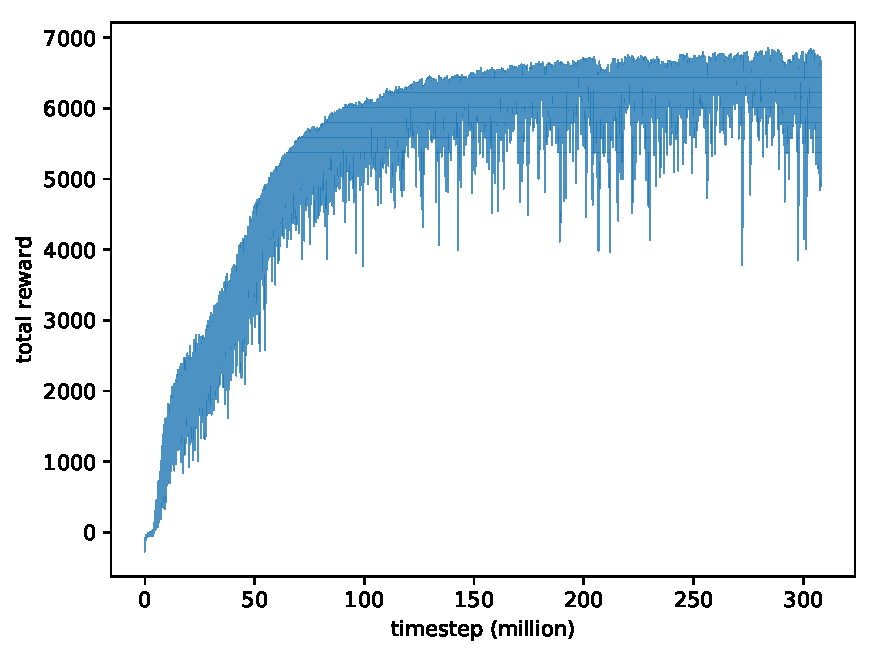
\includegraphics[width=0.7\textwidth]{rec_180608_wass_decay}
	\centering
	\caption{Performance of a W-KTR agent with a decaying W2-metric from 0.02 to 0.00003 in the first 15 million time-steps. The agent is trained with batch-size 4000 and 20 parallel agents. The vertical axis is the total return averaged over the recent 20 episodes and the horizontal axis is the number of million time-steps}\label{fig_wass_decay}
\end{figure}

The experiment results show that the proposed W-KTR algorithm is able to achieve the same level of final performance as the contemporary state-of-art methods. The major drawback is that the algorithm does not perform well in training time. The decaying learning rate feature of KL-divergence based trust region algorithms is able to achieve a proper performance improvement rate in the early phase of training.
%%!TEX program = xelatex
%!TEX root = ./thesis.tex
\section{Solution to the basic environment: \textit{move0}}
In this section, we compare the proposed W-KTR method with other state-of-art algorithms on the basic \textit{move0} environment.

The performance of W-KTR algorithm is shown in Figure \ref{rec_move0_wktr_tune}:

\begin{figure}[h]
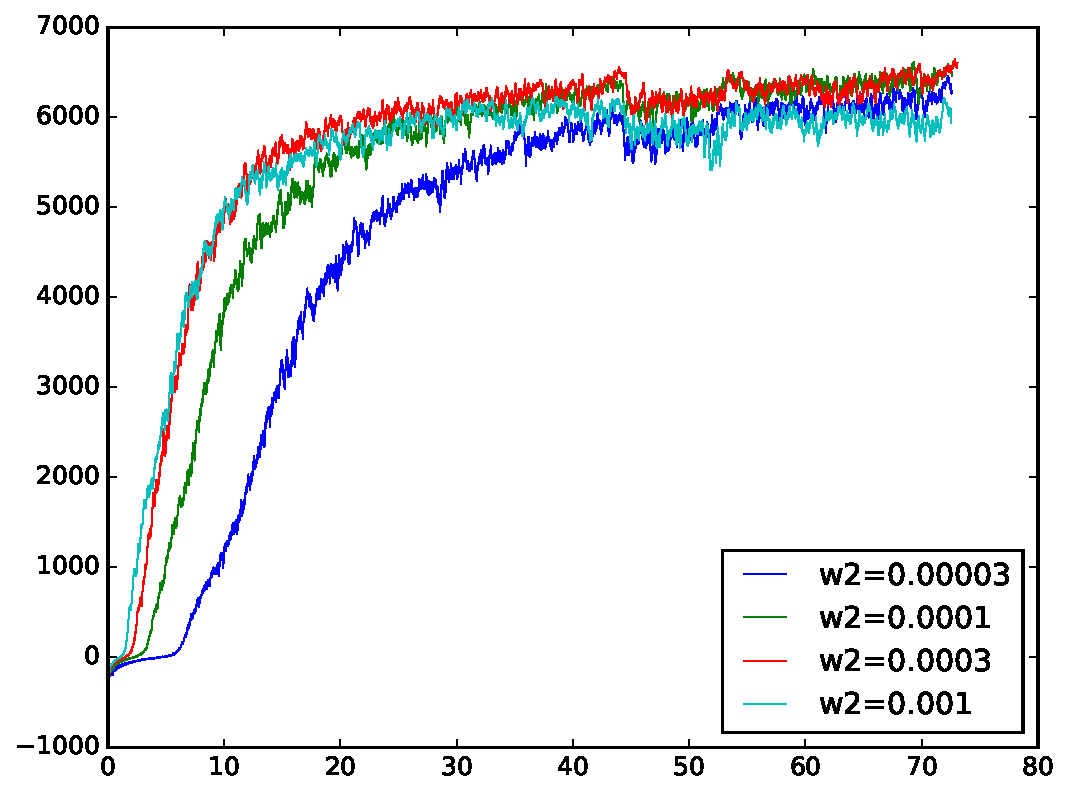
\includegraphics[width=\textwidth]{images/rec_move0_wktr_tune.pdf}
\centering
\caption{Performance of move0 W-KTR agent with diferent hyper-parameter $\delta_W^2$, the x-axis is the number of million timesteps and the y-axis is the total episode reward averaged over the last 200 episodes}
\end{figure}\label{rec_move0_wktr_tune}
It can be shown that the W-KTR agent has a stable final performance, which is not much dependent on the hyper-parameter $\delta_W^2$.

The performance of ACKTR agents is shown in Figure \ref{rec_move0_acktr_tune}:
\begin{figure}[h]
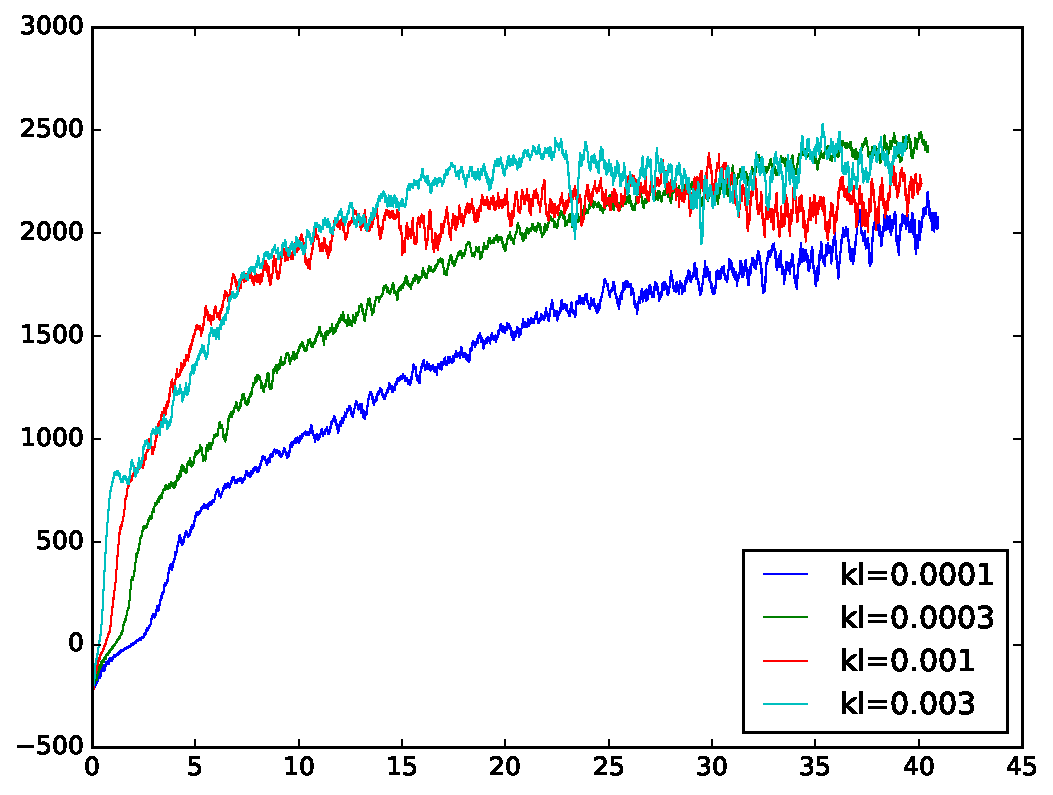
\includegraphics[width=\textwidth]{images/rec_move0_acktr_tune.pdf}
\centering
\caption{Performance of move0 PPO agent with diferent hyper-parameter $\delta_{kl}$, the x-axis is the number of million timesteps and the y-axis is the total episode reward averaged over the last 200 episodes}
\end{figure}\label{rec_move0_acktr_tune}
It can be shown that the ACKTR agent can achieve a faster rate of improvement at the first 10 million steps, but the improvement rate becomes slow as the training proceeds. The agents tend to stuck at sub-optimal policies since the policies converge too fast and cannot effectively adjust once the STD becomes small.

We also run experiments on tuning a PPO agent for the task move0, which is shown in Figre~\ref{rec_move0_ppo_tuning}. The original PPO algorithms has 40 minibatch updates in each batch, which converges too early. We only performa one gradient update over the whole batch in this experiment. The performance of the PPO agent appears to be sensitive to the hyper-parameter, and the agent can't avoid the drop of performance in the late phase of training. The method also needs to trade-off between the early improvement rate and the final performance. In conclusion, the PPO method is not a robust algorithm.
\begin{figure}[h]
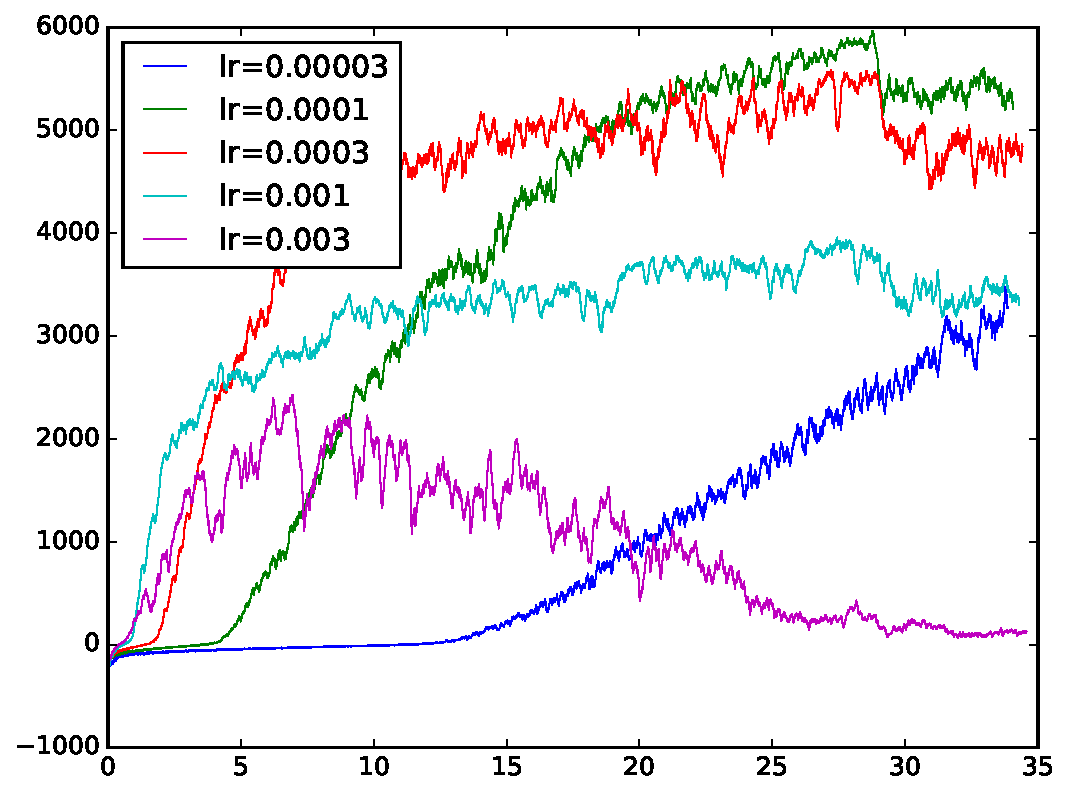
\includegraphics[width=\textwidth]{images/rec_move0_ppo_tuning.pdf}
\centering
\caption{Performance of move0 PPO agent with diferent hyper-parameter $learning rate$, the x-axis is the number of million timesteps and the y-axis is the total episode reward averaged over the last 200 episodes}
\end{figure}\label{rec_move0_ppo_tuning}

All the method above use a batch size of 4000 timesteps produced by 20 parallel agents.

\section{Flat solution to a simple Multi-Modality environment: \textit{move1d}}
In the move1d environment, the agent needs to learn from the image input to decide whether to move forward or backward, as well as control according to the states.
We have tried to solve the problem using ACKTR method, presented in Figure~\ref{rec_flatmove1d_acktr_tune}, shows that the agent can easily get stuck at the score of 1000, and cannot improve much even if the agent breaks the bottleneck because the average STD parameter already drops to below 0.04.
\begin{figure}[h]
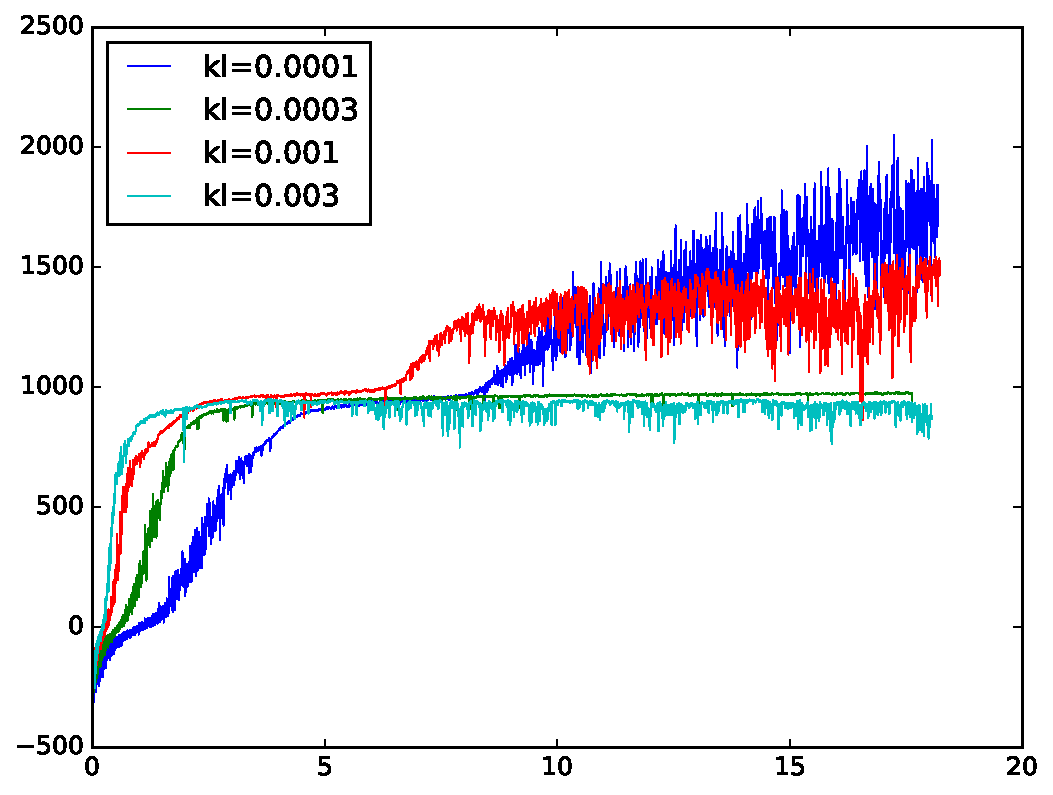
\includegraphics[width=\textwidth]{images/rec_flatmove1d_acktr_tune.pdf}
\centering
\caption{Performance of move1d ACKTR agent with diferent hyper-parameter $learning rate$, the x-axis is the number of million timesteps and the y-axis is the total episode reward averaged over the last 20 episodes}
\end{figure}\label{rec_flatmove1d_acktr_tune}

We also did a single experiment using the proposed W-KTR method, and is shown in Figure~\ref{rec_flatmove1d_wktr}. The W-KTR agent manages to achieve a fast improvement rate and high final performance after getting stuck at the bottleneck score 1000 for a while.
\begin{figure}[h]
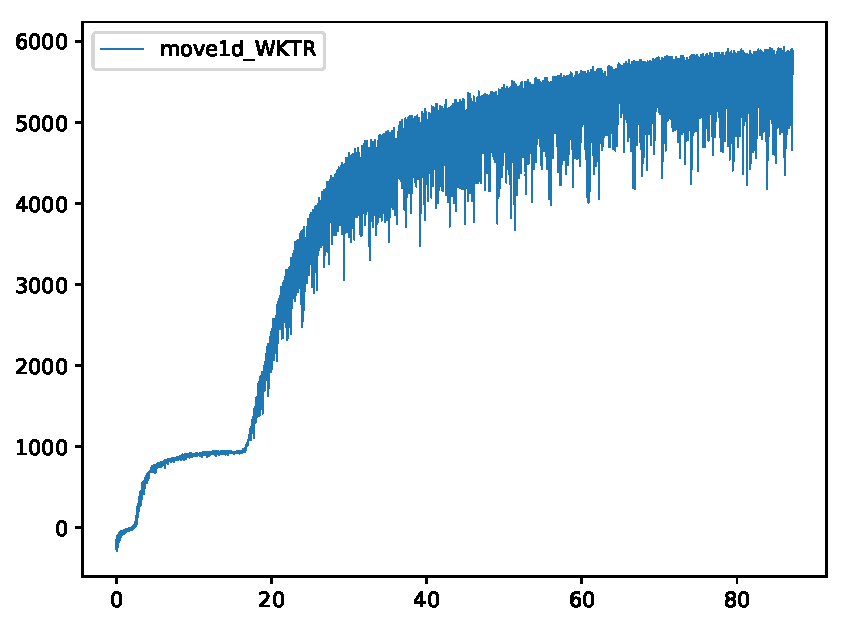
\includegraphics[width=\textwidth]{images/rec_flatmove1d_wktr.pdf}
\centering
\caption{Performance of move1d W-KTR agent with  hyper-parameter $\delta_W^2= 0.0001$, the x-axis is the number of million timesteps and the y-axis is the total episode reward averaged over the last 20 episodes}
\end{figure}\label{rec_flatmove1d_wktr}

This proves that the W-KTR agent is better at handle local minimum and re-adjust the agent's policy even when the policy STD becomes low.



%!TEX program = xelatex
%!TEX root = ./thesis.tex

\section{Experiment on the flat reinforcement learning solution to multi-modality tasks}
\subsection{Discussion on conventional flat reinforcement learning methods}
We observe contemporary end-to-end flat reinforcement learning methods fail to achieve good performance. We suggest that one of the important reason is the image features are much harder to learn than the state. The agent would tend to stuck at a local minimum when it has already learned the state features well, but has not been able to extract any useful information from the image. However, when the agent has finally learned the image features, the policy already converge to a relatively low-entropy distribution, and contemporary reinforcement learning methods cannot perform exploration again at this phase.

We take the task "movecont" as an example. In this task, a goal direction as sampled uniformly at random from the continuous range of angles: $[0,2\pi)$, at the beginning of each episode. The agent can only indicate the goal direction from the image, where there is a sphere object at the corresponding position.

A conventional method for encouraging exploration of reinforcement learning agents with continuous action space is entropy regularization. As we discussed in the section~\ref{sec_method_expadv_reg}, the entropy regularization method is not an effective method in the general case because it simply adds constant biases on the policy parameters and may dominate the learning of the original task.

An experiment on the effectiveness of entropy regularization is shown in Figure~\ref{rec_ent_reg}. The agents are trained using ACKTR algorithm with 32 parallel agents, minibatch-size 2560 and KL-divergence constraint 0.0003. The result shows that the agent easily fails to learn the original task when the weight on entropy term is too large. 

The change of average Standard Deviation of the policy distributions is shown in Figure~\ref{rec_std_ent_reg}. The agents' policy distributions appear to get stuck at certain level of standard deviation when the entropy term is not optimal.
\begin{figure}[!htbp]
	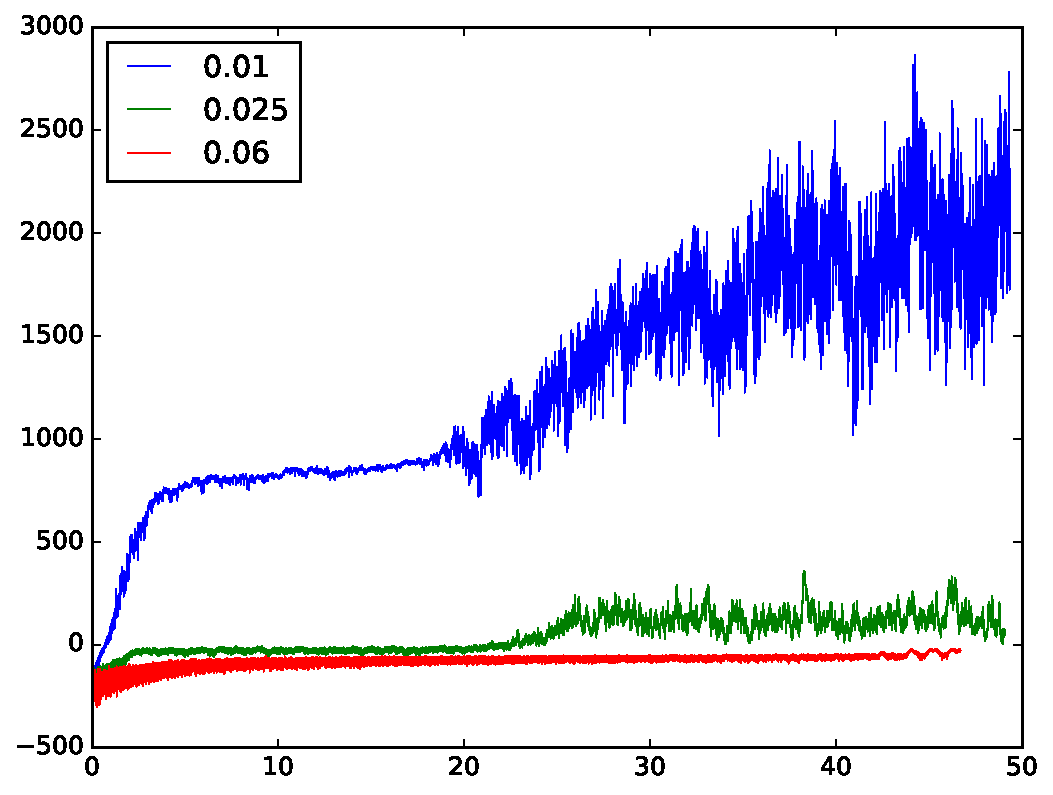
\includegraphics[width=\textwidth]{images/rec_ent_reg.pdf}
	\centering
	\caption{Performance of agents with different weight on entropy regularization term, the horizontal axis is the number of million timesteps and the vertical axis is the total episode reward averaged over the last 32 episodes}\label{rec_ent_reg}
\end{figure}

\begin{figure}[!htbp]
	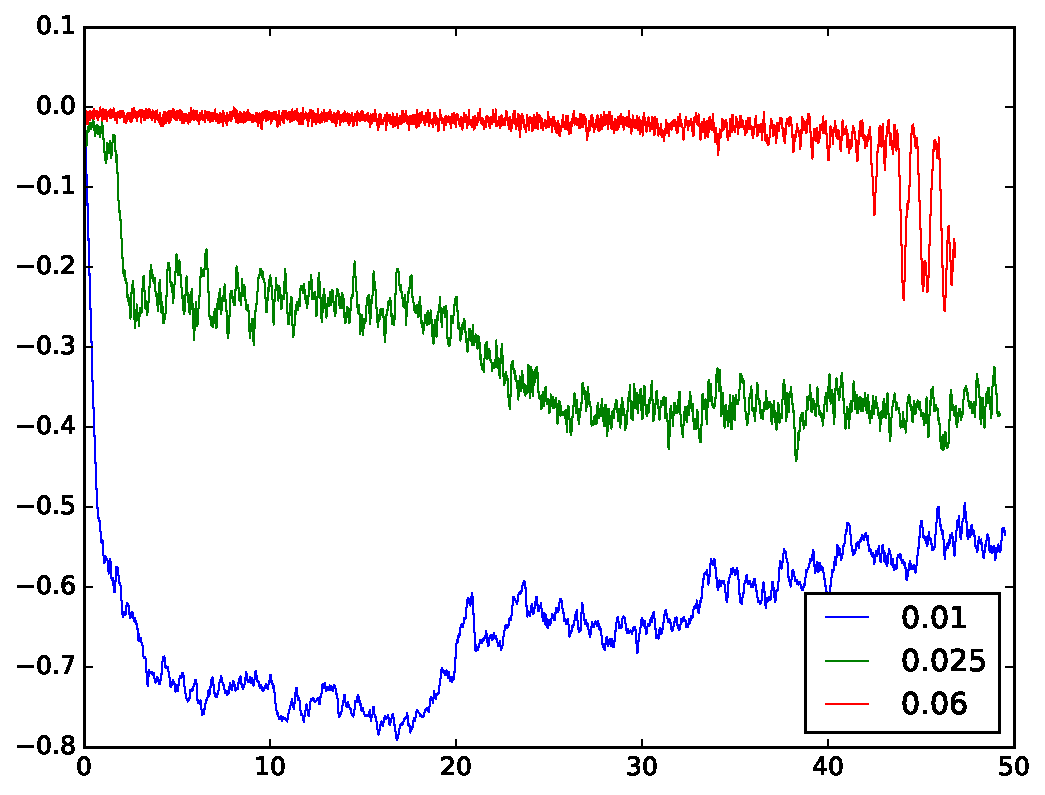
\includegraphics[width=\textwidth]{images/rec_std_ent_reg.pdf}
	\centering
	\caption{Logarithm of average standard deviation of the policy of agents in Figure~\ref{rec_ent_reg}, the horizontal axis is the number of million timesteps.}\label{rec_std_ent_reg}
\end{figure}

\subsection{Experiment on exceptional advantage regularization}
We discuss the effectiveness of exceptional advantage regularization method on multi-modality tasks in this section.

We first demonstrate the general patterns of the distribution on the advantage values on the simple multi-modality task "moveg2". In this task, the goal direction is sampled from 2 opposite directions. The task is much more simple than the "movecont" task because the agent only needs to learn from the image whether it needs to go forward or backward. 

The performance on the total return of an ACKTR agent is shown in Figure~\ref{rec_stat_moveg2}. The performance in terms of average reward per time-step is shown in Figure~\ref{rec_stat_moveg2_meanrt}, and the average standard deviation is shown in Figre~\ref{rec_stat_moveg2_std}.


\begin{figure}[!htbp]
	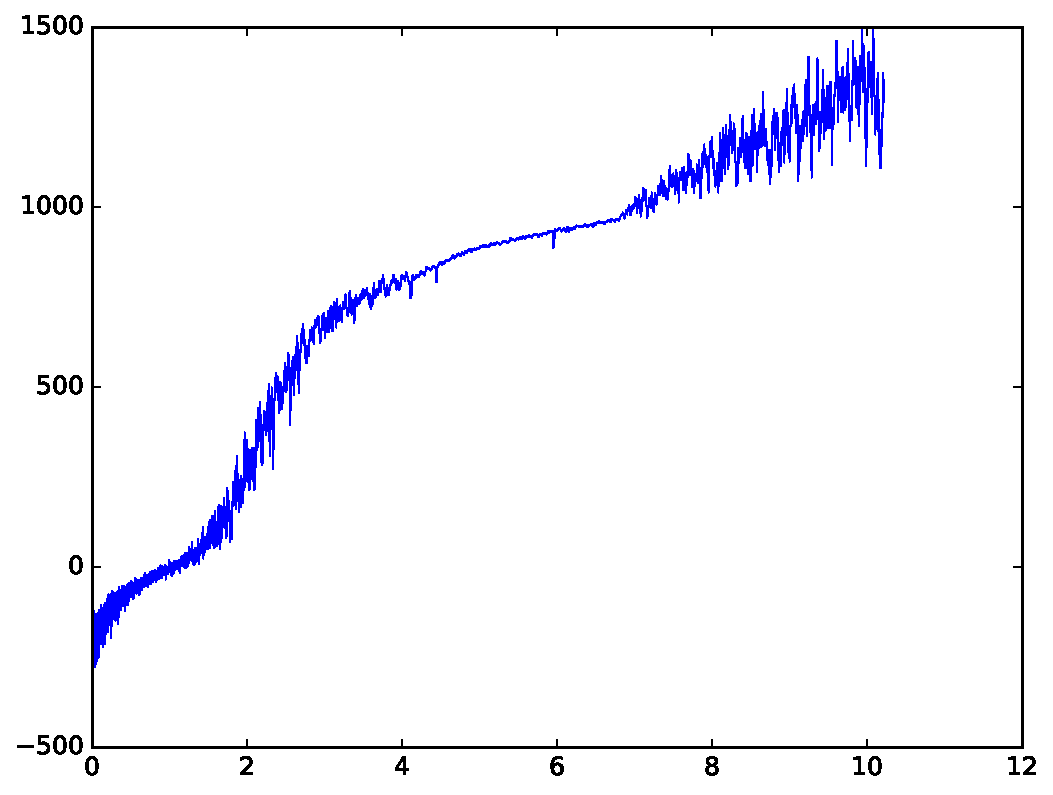
\includegraphics[width=0.7\textwidth]{images/rec_stat_moveg2.pdf}
	\centering
	\caption{Performance of ACKTR agent on the "moveg2" task, the horizontal axis is the number of million timesteps and the vertical axis is the total episode reward averaged over the last 20 episodes}\label{rec_stat_moveg2}
\end{figure}

\begin{figure}[!htbp]
	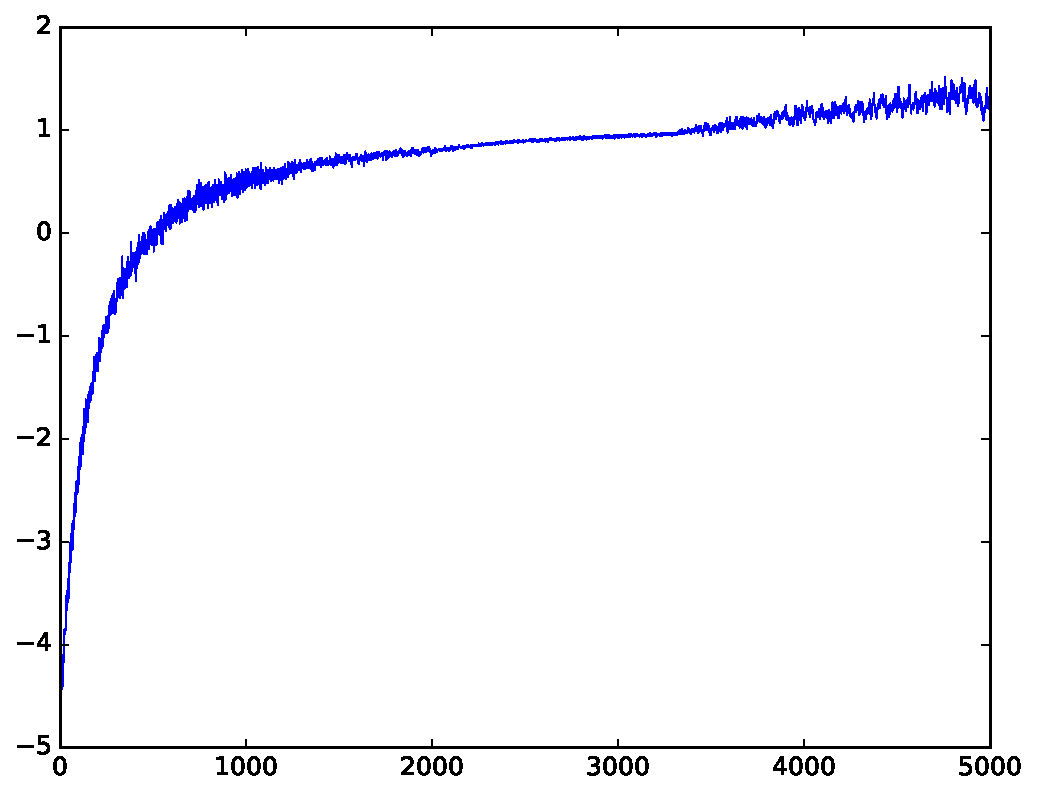
\includegraphics[width=0.7\textwidth]{images/rec_stat_moveg2_meanrt.pdf}
	\centering
	\caption{The avearge reward per time-step of ACKTR agent on the "moveg2" task, the horizontal axis is the number of training batches}\label{rec_stat_moveg2_meanrt}
\end{figure}

\begin{figure}[!htbp]
	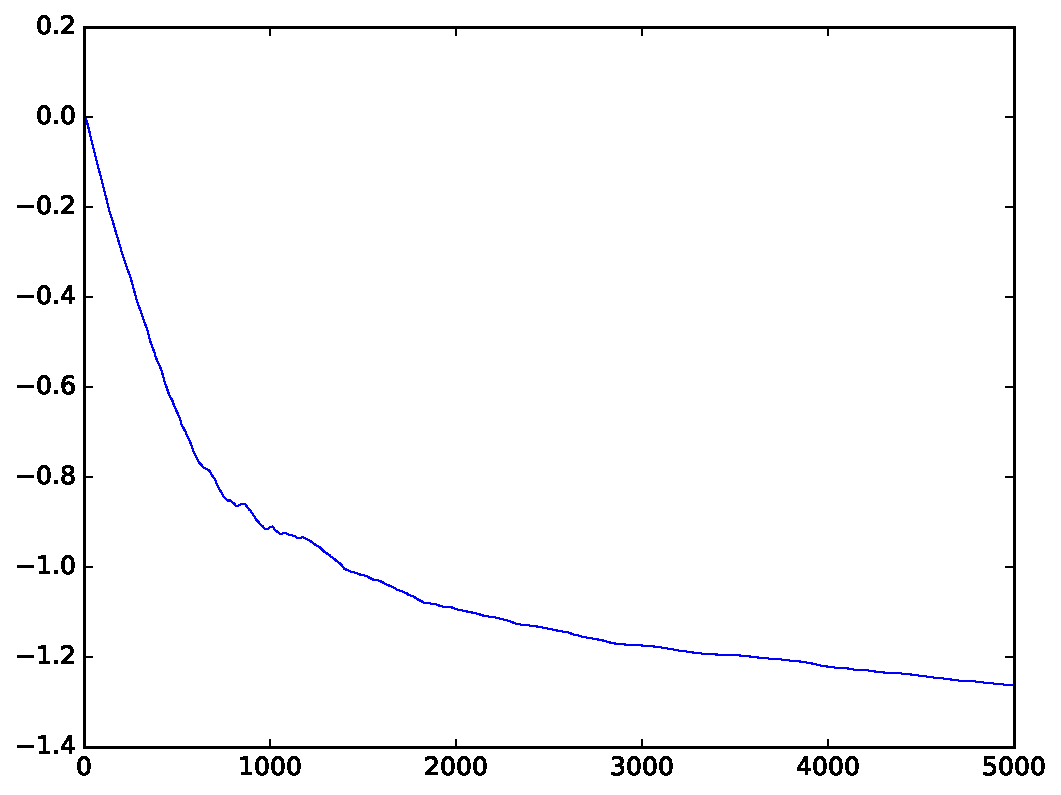
\includegraphics[width=0.7\textwidth]{images/rec_stat_moveg2_std.pdf}
	\centering
	\caption{The logarithm of avearge standard deviation of ACKTR agent's policy on the "moveg2" task, the horizontal axis is the number of training batches}\label{rec_stat_moveg2_std}
\end{figure}
The distribution of advantage values at the first batch (batch 0) is shown in Figure~\ref{vis_stats_0}. It can be seen that the advantage values are distributed uniformly across different values of log-likelihood because the critic model has not been trained. After the critic model has been trained for a reasonable amount of time, the marginal distribution advantage value tend to follow a normal distribution with zero mean. An example is shown in Figure~\ref{vis_stats_3000}, which is the distribution at batch 3000. However, the advantage values are likely to have higher values at low log-likelihood samples when the agent has just escaped from a local minimum. An example is Figure~\ref{vis_stats_4900}, which shows the the distribution of advantage values at batch 4900. It can be seen that the distribution becomes significantly different because many positive advantage points are spread across different log-likelihoods. 

Intuitively, a large number of points with low log-likelihood but high advantage value indicates that the agent needs to increase the degree of exploration. However, the figure~\ref{rec_stat_moveg2_std} on the change of standard deviation shows that the agent actually still keep decreasing the standard deviations of its policy even at this state. Therefore, the application of a exceptional advantage regularization term, could be useful in encouraging exploration in these cases.

\begin{figure}[!htbp]
	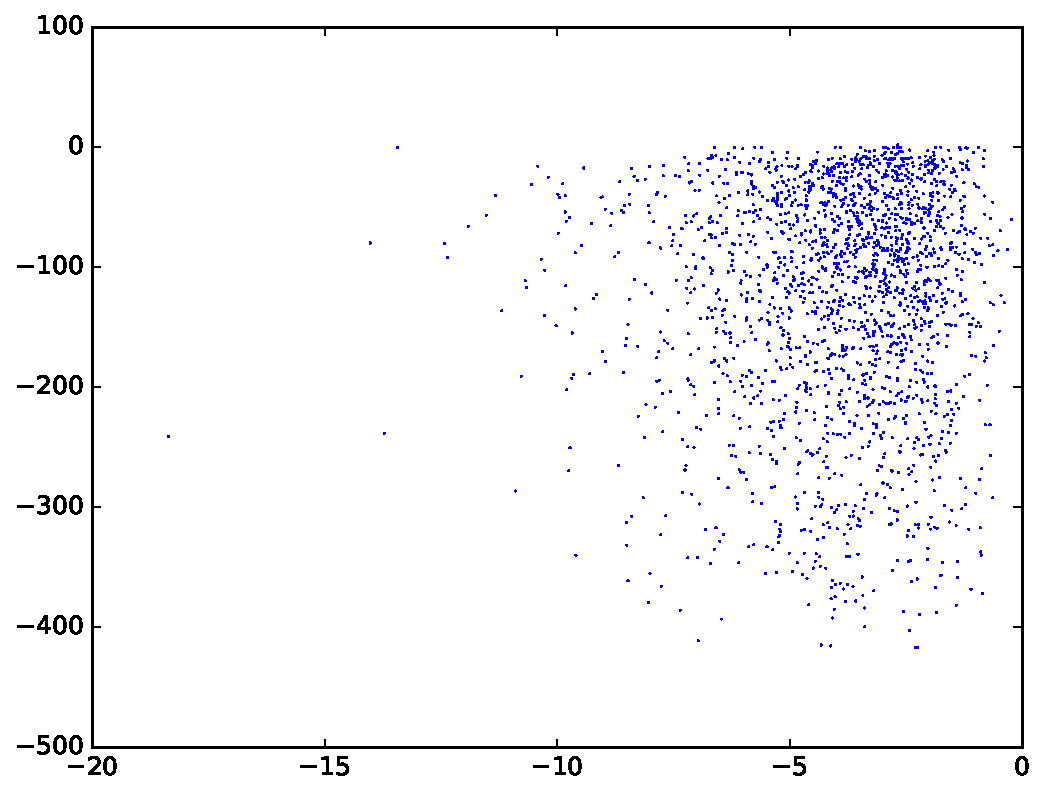
\includegraphics[width=\textwidth]{images/vis_stats_0.pdf}
	\centering
	\caption{The distribution of advantage values of the ACKTR agent at batch 0 on the "moveg2" task, the horizontal axis is the log-likelihood value}
	\label{vis_stats_0}
\end{figure}

\begin{figure}[!htbp]
	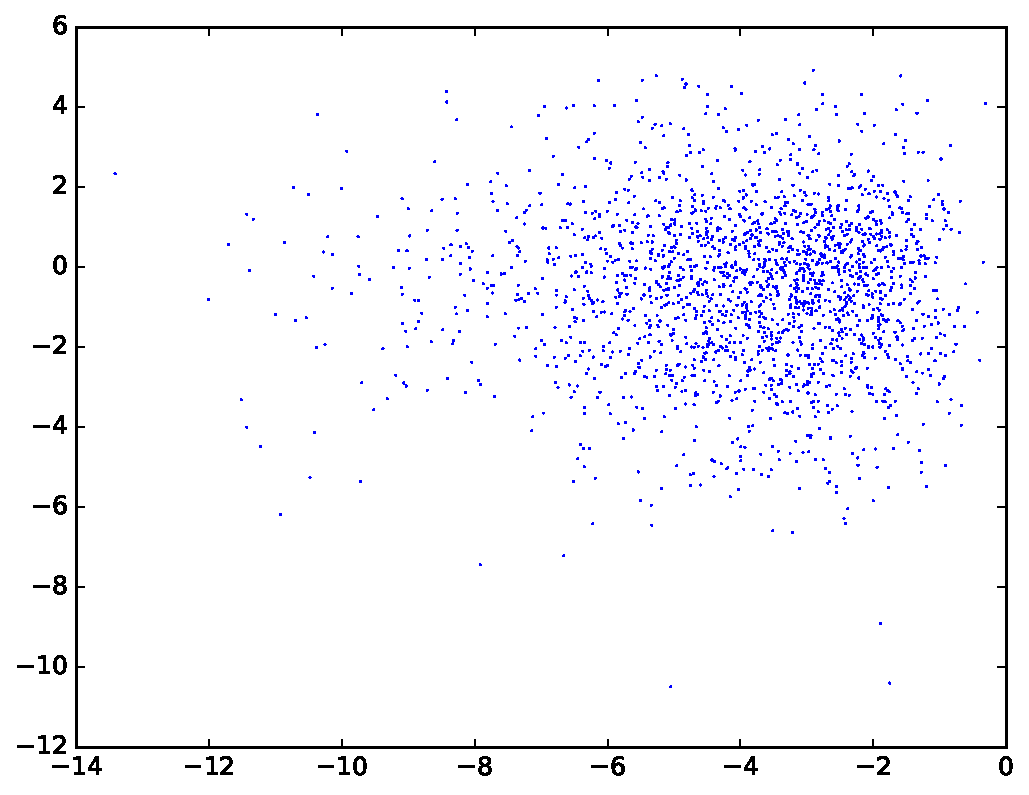
\includegraphics[width=\textwidth]{images/vis_stats_3000.pdf}
	\centering
	\caption{The distribution of advantage values of the ACKTR agent at batch 300 on the "moveg2" task, the horizontal axis is the log-likelihood value}
	\label{vis_stats_3000}
\end{figure}

\begin{figure}[!htbp]
	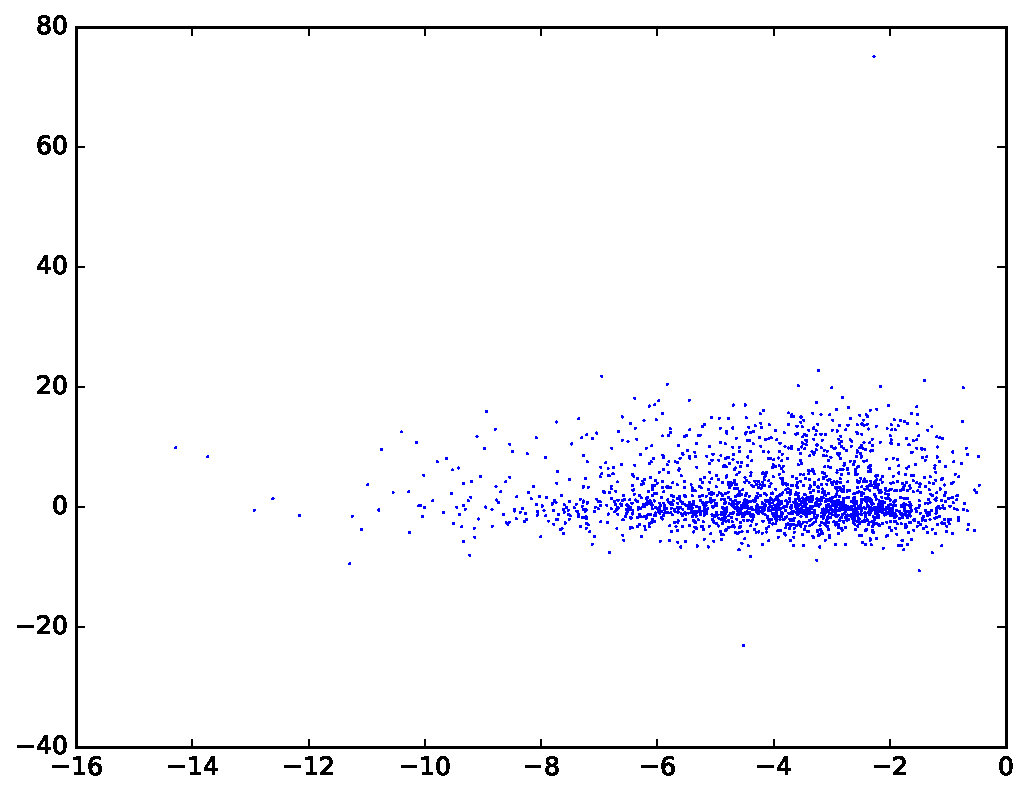
\includegraphics[width=\textwidth]{images/vis_stats_4900.pdf}
	\centering
	\caption{The distribution of advantage values of the ACKTR agent at batch 4900 on the "moveg2" task, the horizontal axis is the log-likelihood value}
	\label{vis_stats_4900}
\end{figure}

We then verify the performance of exceptional advantage regularization on the 'movecont' task.
The performance of an ACKTR agent with different weights exceptional advantage regularization on the in Figure~\ref{rec_adv_reg}, and the average standard deviation parameter of their policies are shown in Figure~\ref{rec_std_adv_reg}. All the agents are trained with batch-size 2560 and KL-divergence constraint 0.0003. The weight-0 agent is the same as the original ACKTR agent without any exploration regularization, and it could only achieve a total reward of around 2000 at the end of training. The agent with exceptional advantage regularization weight 0.04 can improve rapidly in the early phase before 40 million timestep, but gets stuck at around 3500. This shows that the exceptional advantage regularization method could have adverse effect on the convergence of policy in the late phase of training, which is also indicated in by average std curve. The agent with exceptional advantage regularization weight 0.01 achieves the best final performance. Its average standard deviation shows that the agent manages to increase its policy entropy and re-explore the environment after it has escaped from a local minimum.
\begin{figure}[!htbp]
	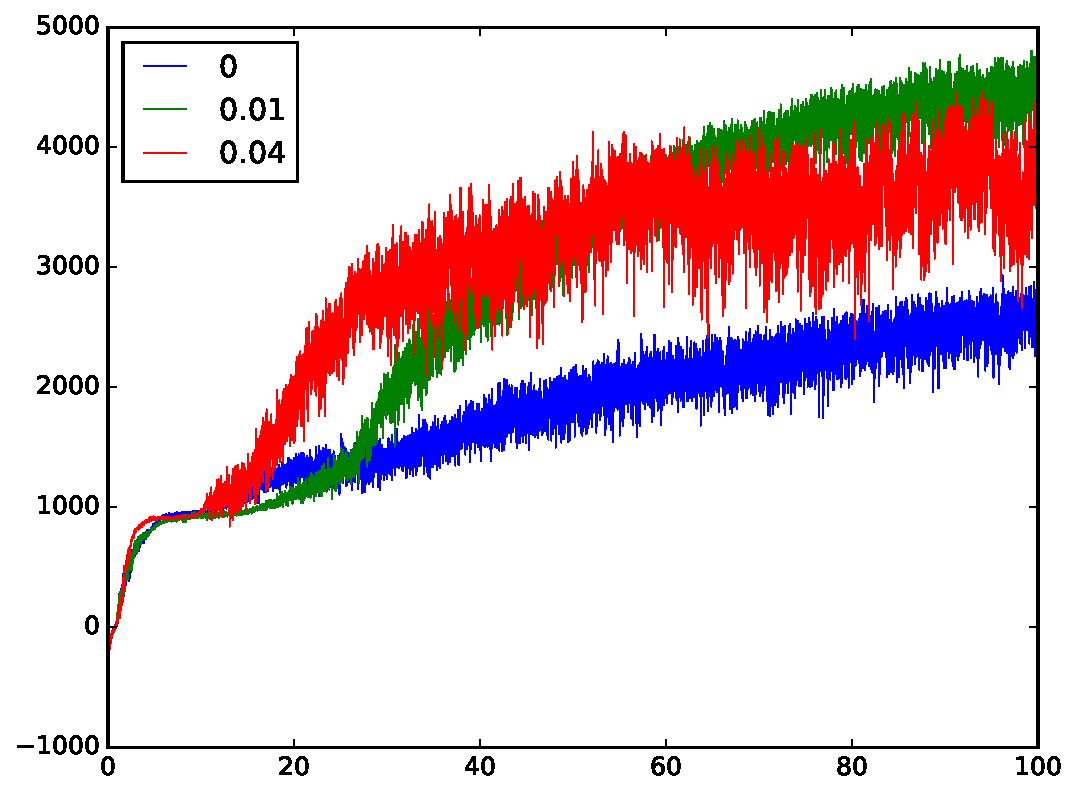
\includegraphics[width=\textwidth]{images/rec_adv_reg.pdf}
	\centering
	\caption{Performance of agents with different exceptional advantage regularization weights, the x-axis is the number of million time-steps and the y-axis is the total episode reward averaged over the last 32 episodes}\label{rec_adv_reg}
\end{figure}

\begin{figure}[!htbp]
	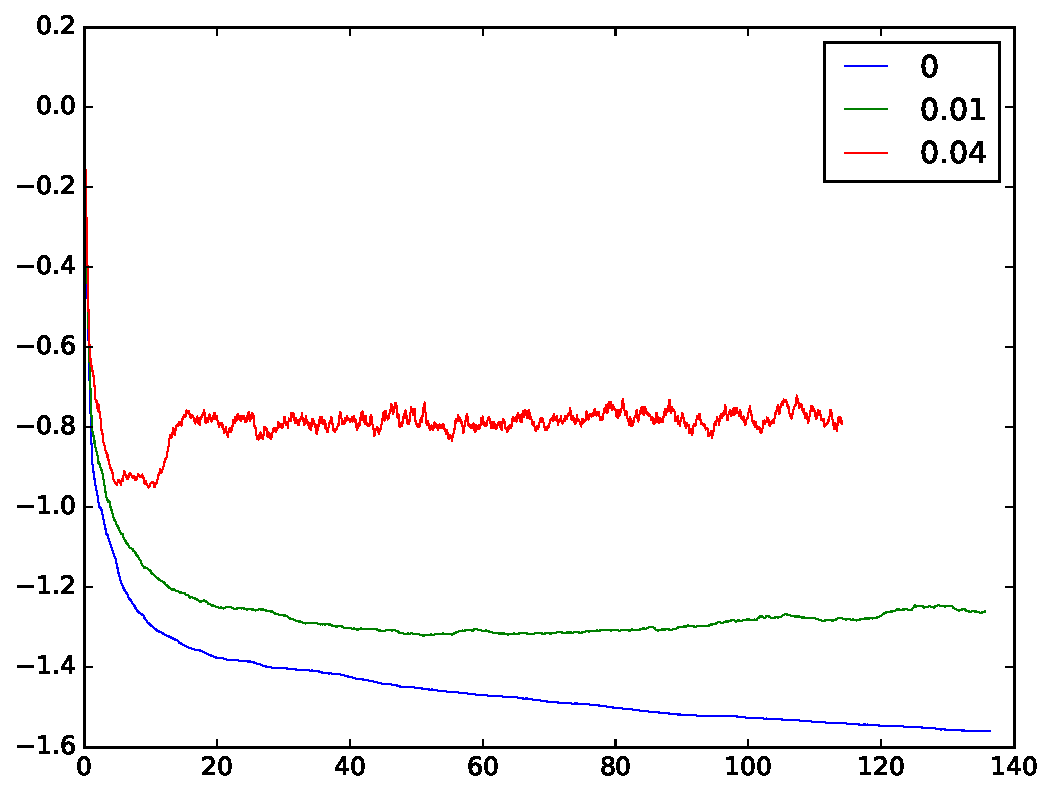
\includegraphics[width=\textwidth]{images/rec_std_adv_reg.pdf}
	\centering
	\caption{The logarithm of avearge standard deviation of agents with different exceptional advantage regularization weights, the horizontal axis is the number of million time-steps and the vertical axis is the total episode reward averaged over the last 32 episodes}\label{rec_std_adv_reg}
\end{figure}

\subsection{Experiment on the Robust Concentric Mixture Gaussian Policy}
The effectiveness of robust concentric mixture Gaussian policy agent in exploration of task "movecont" is verified in this section. 

The performance of an ACKTR mixture Gaussian policy agent is shown in Figure~\ref{rec_mix}. The results shows that the mixture Gaussian policy agents have slower learning rates compared to pure Gaussian policy agents. However, the agents are able to achieve a good fubak performance, with a total reward of around 4000 when the KL-divergence is set properly.

\begin{figure}[!htbp]
	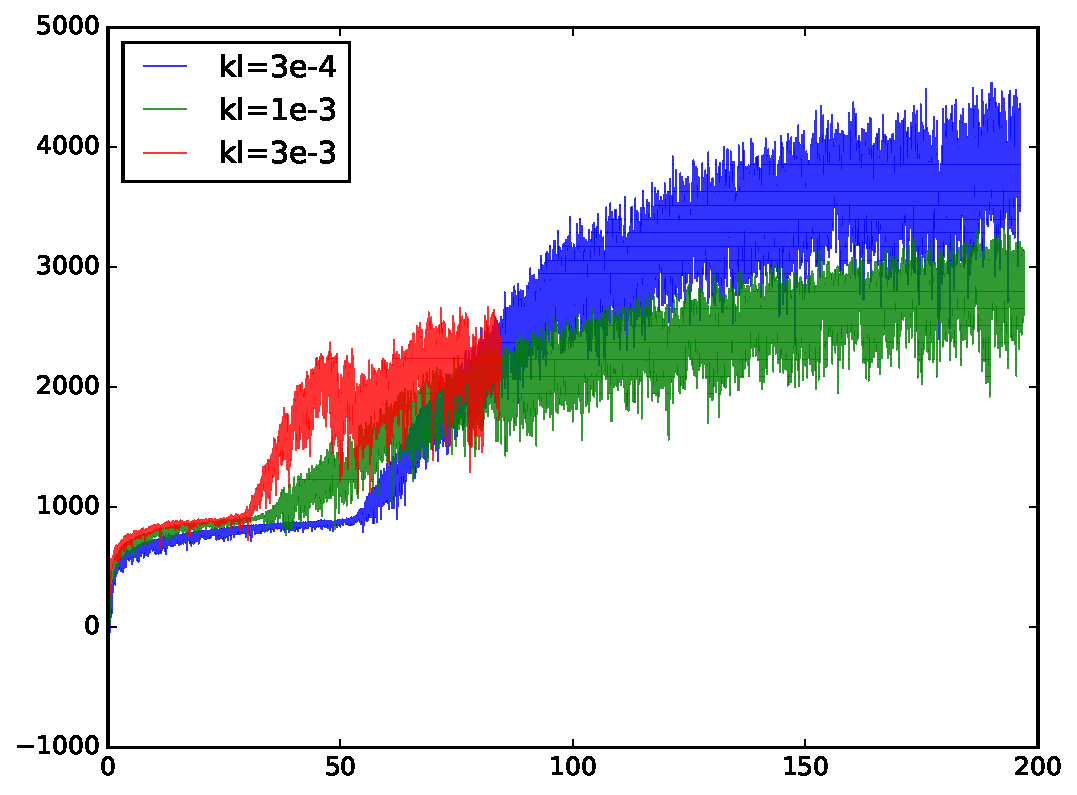
\includegraphics[width=\textwidth]{images/rec_mix.pdf}
	\centering
	\caption{Performance of ACKTR agents with different KL-divergence constraints, the x-axis is the number of million time-steps and the y-axis is the total episode reward averaged over the last 32 episodes}\label{rec_mix}
\end{figure}

%!TEX program = xelatex
%!TEX root = ./thesis.tex

\section{Hierarchical reinforcement learning methods for multi-modality and sparse environments}
This section will discuss the experiments on the proposed hierarchical reinforcement learning models.

In our experiment settings, we choose the set $\{move0, move1, \dots, move7 \}$ as source tasks. We select "dynamicg4" as a representative target task for multi-modality environments and "reachcont" as a representative target task for multi-modality sparse environments.

The problem of hierarchical reinforcement learning is divided into two parts: learning robust actuator policies and learning the decider policies. The following two section will discuss these two problems.


\subsection{Training of actuator agents with Domain randomization by cross-sampling initial states}
We examine the performance of domain randomization by cross-sampling initial states in this section. A visualization on on an experiment on the domain randomization by cross-sampling initial states method on the set of source tasks $\{move0, move1, \dots, move7 \}$ is shown in Figure~\ref{rec_8task_training}.

The result shows that the agents produce different final performance levels, despite that all the actuator agents are basically learning the same type of task. This shows that the collective training of actuator policies suffers from "strategy collapse".

\begin{figure}[!htbp]
	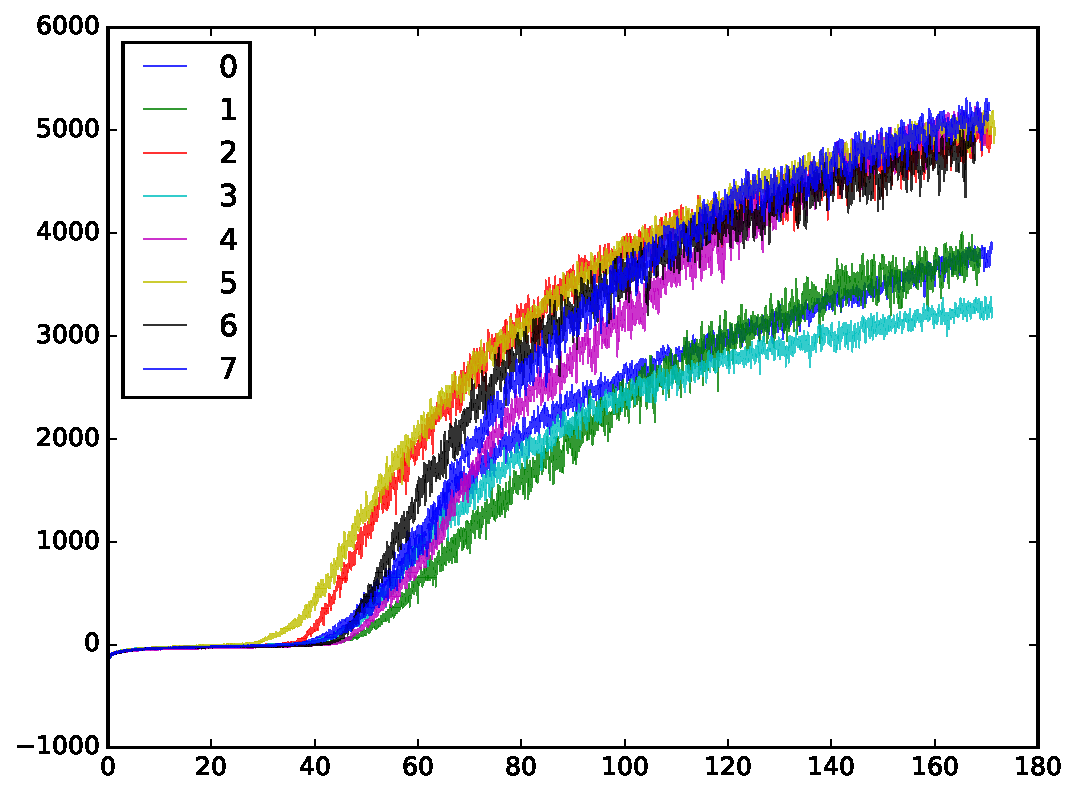
\includegraphics[width=\textwidth]{images/rec_8task_training.pdf}
	\centering
	\caption{Performance of actuator agents with domain randomization by cross-sampling initial states, the x-axis is the number of million time-steps and the y-axis is the total episode reward averaged over the last 200 episodes}\label{rec_8task_training}
\end{figure}

The experiment results of the proposed "synchronous scheduling of actuator learning" is shown in Figure \ref{rec_sync_training}. In this experiments, the agents who outperforms the global lowest-performance by 1000 is paused until it becomes the agent with the lowest performance. The result shows that all the actuator agents reach a final performance of around 6000 although their performance diverge initially.

\begin{figure}[!htbp]
	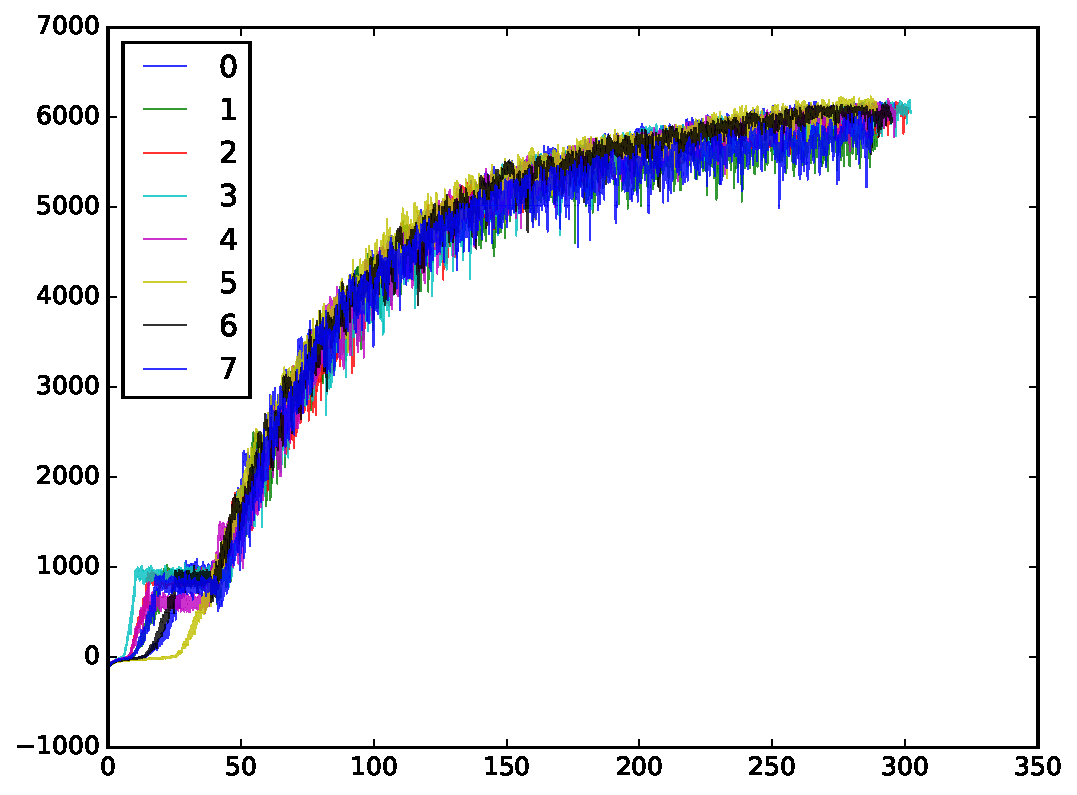
\includegraphics[width=\textwidth]{images/rec_sync_training.pdf}
	\centering
	\caption{Performance of actuator agents using "synchronous scheduling of actuator learning" , the x-axis is the number of million time-steps and the y-axis is the total episode reward averaged over the last 200 episodes}\label{rec_sync_training}
\end{figure}

\subsection{Training of decider agent}
The experiment on the training of decision policy on "dynamicg8" is shown in Figure~\ref{fig:rec_dynamicg8_decider_subt10}. %TODO

\begin{figure}[!htbp]
\centering
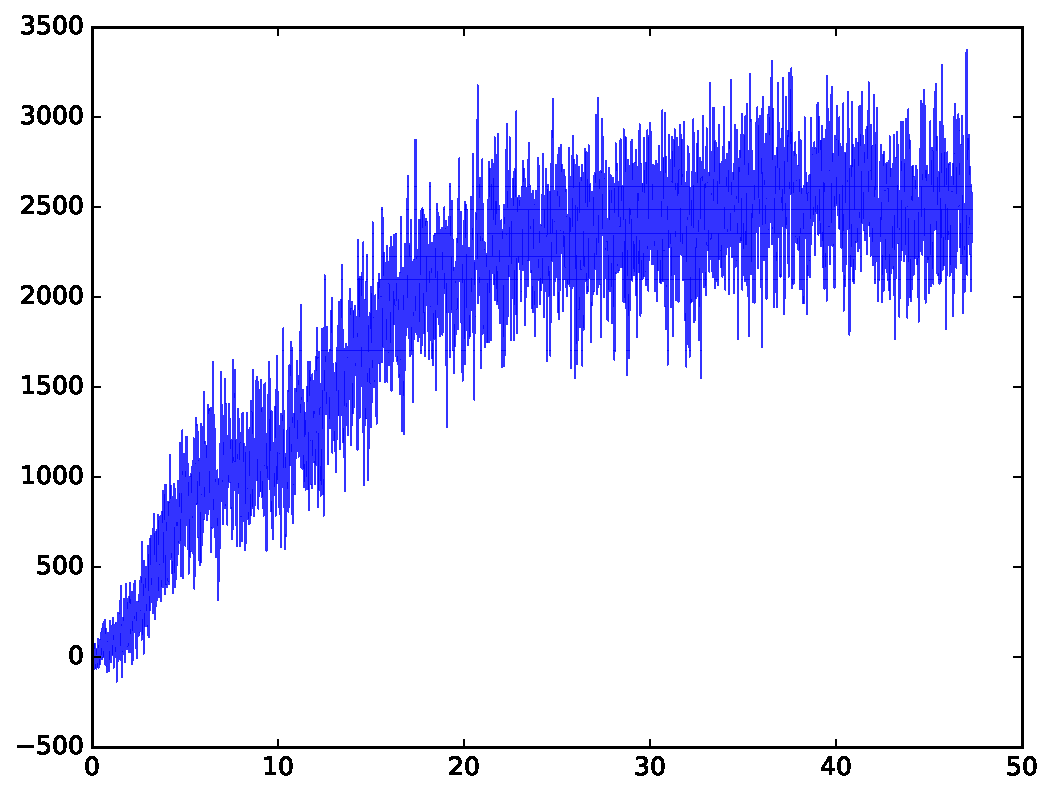
\includegraphics[width=\linewidth]{rec_dynamicg8_decider_subt10}
\caption{Decision policy training performance of the task "dynamicg8", the x-axis is the number of million time-steps and the y-axis is the total episode reward averaged over the last 32 episodes}
\label{fig:rec_dynamicg8_decider_subt10}
\end{figure}

The experiment on the training of decision policy on task "reachcont" is shown in Figure~\ref{fig:rec_reachc05_decider_subt10}.
\begin{figure}
\centering
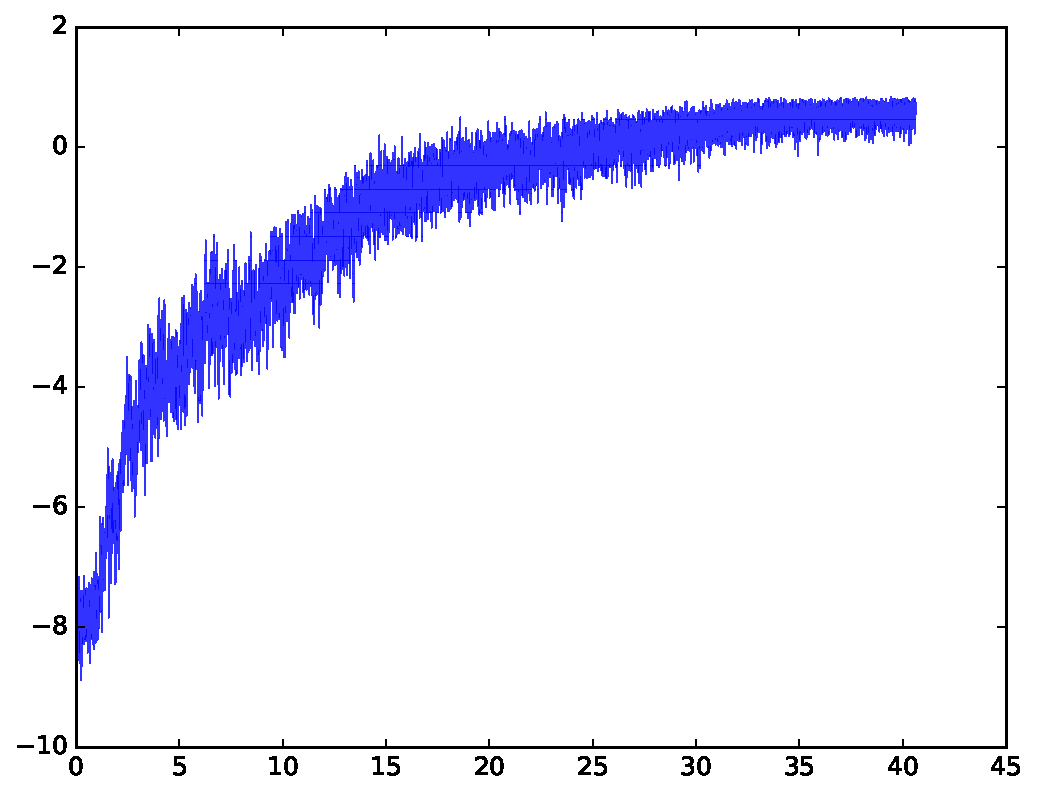
\includegraphics[width=1\linewidth]{rec_reachc05_decider_subt10.pdf}
\caption{}
\label{fig:rec_reachc05_decider_subt10}
\end{figure}



% \section{Preliminary experiment on the hierarchical agent architecture}
% A preliminary experiment has been done on training the proposed agent in the dynamic2d environment. The termination policy sets $b_i = 4.5$ and isn't trained during policy updates. The figure is shown in Figure \ref{rec_180419_fix_ter}.

% The result shows that the learning of the root-level policy is effective.


% \begin{figure}[h]
% 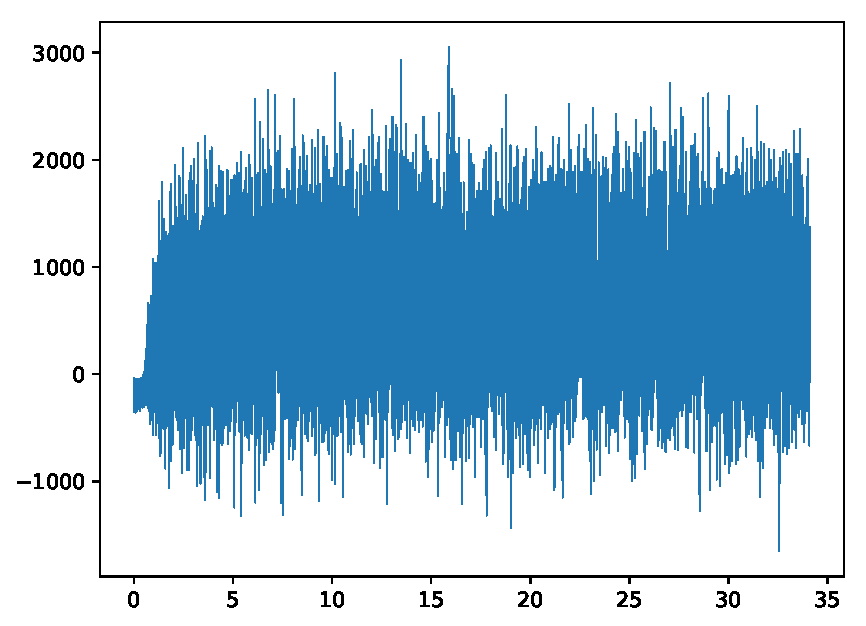
\includegraphics[width=\textwidth]{images/rec_180420_fix_ter.pdf}
% \centering
% \caption{Experiment on dynamic2d on a hierarchical reinforcement learning agent with fixed-length termination policy}
% \end{figure}\label{rec_180419_fix_ter}

% The current guess on the source of stability is that the sub-policy doesn't perform well in the target environment. Figure \ref{rec_180419_fix_ter_len} shows the average episode length of the hierachical agent.

% \begin{figure}[h]
% 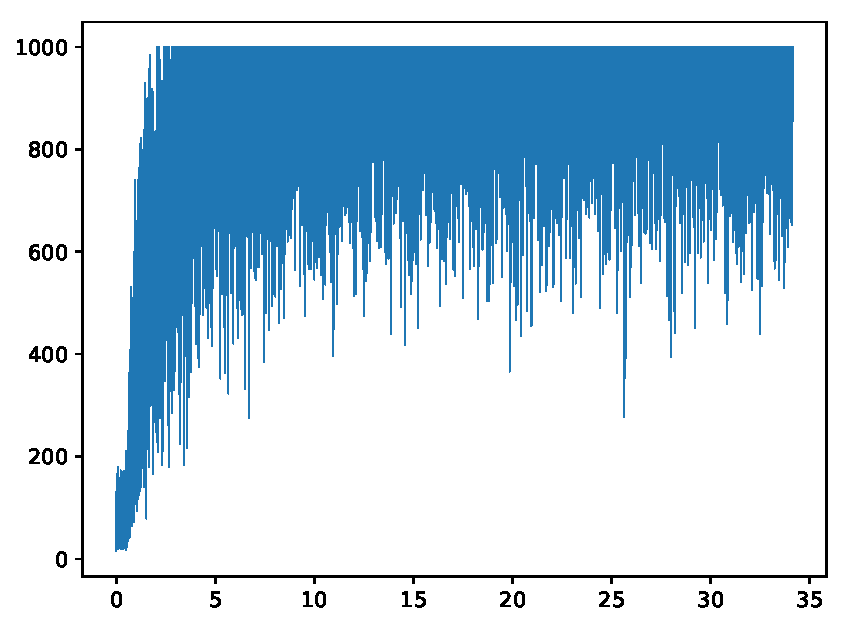
\includegraphics[width=\textwidth]{images/rec_180420_fix_ter_len.pdf}
% \centering
% \caption{The average episode length of the dynamic2d hierarchical agent}
% \end{figure}\label{rec_180419_fix_ter_len}

% \section{Experiment up to April. 26: on transfer of source policies}
% The results show that the source task policy cannot perform well in dynamic2d, because of different initial condition caused by the switching of moving direction.

% An experiment is developed to fine-tune the source task policies during the learning of the target task. However, the problem is on how to fine-tune a Gaussian policy that has already converged with low STD.

% \section{Ongoing development in transfer of actuator policy}
% \section{On training source tasks}
% I found that using a 1-step proximate policy gradient algorithm with an adaptive KL penalty is the most economic method.

% Previously, the ACKTR agent sometimes stuck at a performance around 3000 as discussed in the group meeting in March. The reason could be due to KL divergence constraint is too small. A small change in the mean vector could lead to a large KL divergence when the STD converges to nearly zero. That prevents the agent's policy from improving.

% It is likely that an alternative metric could be better for trust region methods, like L1-error or JS-divergence.
% \subsection{Training the actuator policy from scratch in the target task}
% An experiment is being run to test if the agent can effectively learn the actuator policies. The actuator agent learns stably. However the rate of improvement is slow due to the simultaneous training of all the source tasks. The current per step mean reward reaches 1.5 after 3 days.
% \subsection{Fine-tuning the actuator policies}
% The fine-tuning of the actuator polices seems to fail in the target problem. The performance usually drops during the fine-tuning period. 
% Deeper investigations are undergoing to fix the problem.
% \subsection{Training a transition policy}
% The development of the transition policy is still undergoing.
% \section{On the hierarchical reinforcement learning}
% I found that the current scheduler agent model is unstable in training. 

% I'm trying to develop a mixed type policy network, where the output is a binary variable and the discrete/continuous distribution. The binary variable indicates whether the current actuator policy should be terminated, and the latter one denotes the policy distribution. The relevant properties such as KL divergence for this kind of distribution should be derived and developed.

% \section{Progress by May. 10}
% Current work still focuses on the investigation of transferring actuator policies.
% The current model fails to reproduce the previous positive experiments on multi-modality tasks. I've done several bug-fixes and parameter tuning, however the problem still remains. The cause is still under investigation, one possible cause is related to the stability of actuator policies in terms of failure rate. If an actuator policy is prune to "game over" behaviour when initialized after another actuator policy, the decider agent may tend to constantly choose a fixed policy. 

% \section{Progress by Mar. 17}
% \subsection{Reproduction of the multi-modality environment performance}
% I've just finished fixing the code, so that the new model achieves a reasonable performance in move1d. The performance is shown in Figure \ref{rec_move1d}.
% \begin{figure}[h]
% 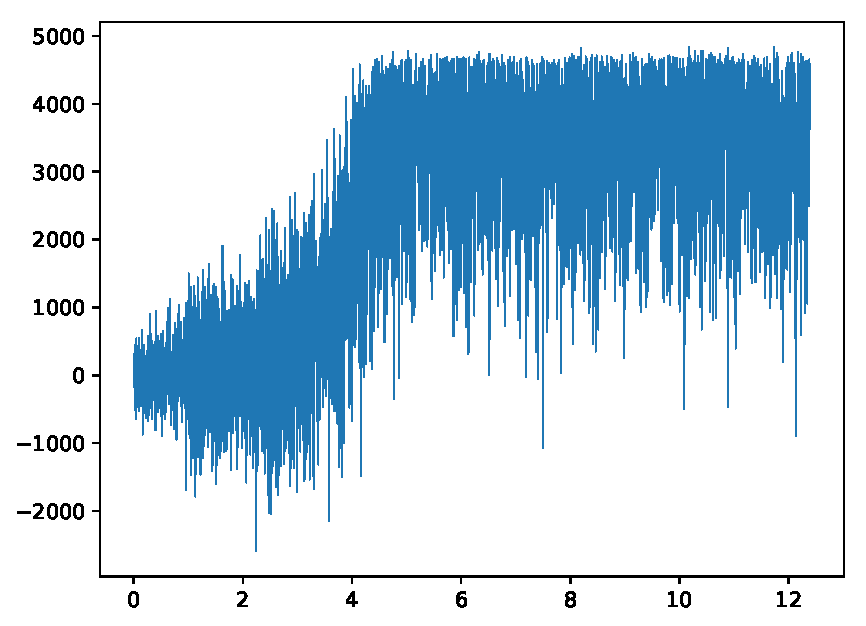
\includegraphics[width=\textwidth]{images/rec_180517_move1d_better.pdf}
% \centering
% \caption{Experiment on move1d}
% \end{figure}\label{rec_move1d}

% \subsection{Study of generalized advantage estimation}
% During the development of the hierarchical reinforcement learning model, I developed a modified version of \cite{schulman2015high} for hierarchical reinforcement learning methods. I found a problem that the original method didn't correctly normalize the advantage values $A_t$ according to $\sum_{i=t}^{i=t+T}\lambda^{i}$. That would lead to a advantage values linearly increasing magnitudes with the increased time to termination. However, I found that the correct method doesn't produce a better result according to the experiments up to now.

% \subsection{Policy gradient methods with Wasserstein metric}
% I found that one problem with the current KL-divergence based trust region methods is that agents will find it difficult to learn after the STD of the Gaussian policy approaches zero, due to the sensitive KL-divergence loss. I found that it seems better to replace the KL-divergence metric with Wasserstein metric for Gaussian policies.

% A preliminary experiment is done on the original Ant task and has shown positive results, which is shown in Figure \ref{rec_wass}. The proposed agent is the policy gradient agent with adaptive Wasserstein metric penalty.

% \begin{figure}[h]
% 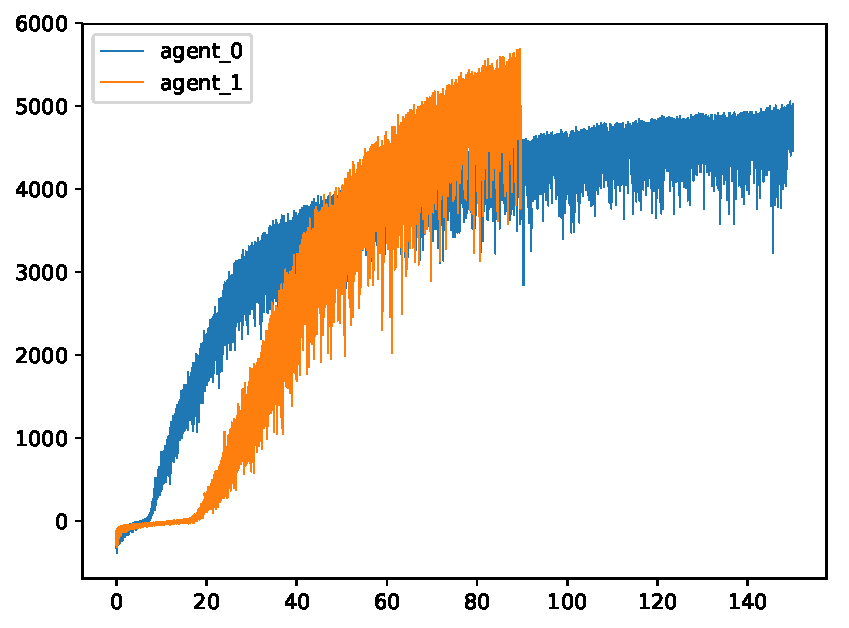
\includegraphics[width=\textwidth]{images/rec_180517_wasserstein.pdf}
% \centering
% \caption{Experiment comparison on Wasserstein metric and KL divergence. agent\_1 is the Wasserstein agent}

% \end{figure}\label{rec_wass}

